\section{Tiles, positive laws, and localization}\label{sec:preliminaries}

Except where an endpoint statement is explicitly made, fix $1\le q<4$ and write
\begin{equation}\label{prelim:parameters}
 d=\sqrt q=2\cos\lambda,\qquad \rho=\lambda/\pi,
 \qquad 0<\lambda\le\pi/3.
\end{equation}
All constants may depend on this fixed parameter and on the fixed geometric
shapes under consideration. In particular, none of the estimates below is
asserted uniformly as $q\uparrow4$.

\subsection{Tiles and boundary caps}

We use a square tile array whose corner sites alternate between primal
($\mathsf P$) and dual ($\mathsf D$) sites. The primal lattice consists of the
primal diagonals, so its mesh is $\sqrt2$ times the tile-edge length. Rotating
the tile coordinates gives the prescribed orientation of the primal square
lattice. Each tile carries one of the two noncrossing pairings of its four
side midpoints, called \emph{ports}. Pairing around the dual corners declares
the primal diagonal open; the other pairing declares the dual diagonal open.
An \emph{actual color path} uses these open diagonals and never uses boundary
identifications as edges. A strand has an actual primal path on one side and
an actual dual path on the other.

\begin{figure}[htbp]
\centering
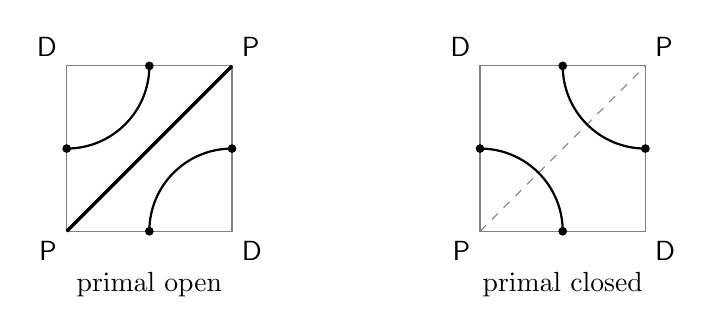
\begin{tikzpicture}[scale=1.05]
 \begin{scope}
  \draw[gray] (0,0) rectangle (2,2);
  \draw[very thick] (0,0)--(2,2);
  \draw[thick] (0,1) arc[start angle=-90,end angle=0,radius=1];
  \draw[thick] (1,0) arc[start angle=180,end angle=90,radius=1];
  \node[below left] at (0,0) {$\mathsf P$};
  \node[above right] at (2,2) {$\mathsf P$};
  \node[above left] at (0,2) {$\mathsf D$};
  \node[below right] at (2,0) {$\mathsf D$};
  \foreach \x/\y in {0/1,1/0,2/1,1/2}
    \fill (\x,\y) circle (1.5pt);
  \node at (1,-.65) {primal open};
 \end{scope}
 \begin{scope}[xshift=5cm]
  \draw[gray] (0,0) rectangle (2,2);
  \draw[dashed,gray] (0,0)--(2,2);
  \draw[thick] (1,0) arc[start angle=0,end angle=90,radius=1];
  \draw[thick] (2,1) arc[start angle=-90,end angle=-180,radius=1];
  \node[below left] at (0,0) {$\mathsf P$};
  \node[above right] at (2,2) {$\mathsf P$};
  \node[above left] at (0,2) {$\mathsf D$};
  \node[below right] at (2,0) {$\mathsf D$};
  \foreach \x/\y in {0/1,1/0,2/1,1/2}
    \fill (\x,\y) circle (1.5pt);
  \node at (1,-.65) {primal closed};
 \end{scope}
\end{tikzpicture}
\caption{The two tile switches. The solid diagonal is an open primal
edge; the dashed diagonal records the absent primal edge. The curved
arcs specify the pairing of ports and hence the order of strand
occurrences when a medial vertex is visited twice.}
\label{prelim:switch-figure}
\end{figure}

For topological arguments, draw the two arcs of a switch disjointly within
its tile, normally to the sides at their ports. This drawing and the straight
medial drawing can be parametrized piece by corresponding piece, preserving
the order of occurrences at a double visit. Their uniform distance is at
most twice the tile diameter. Thus these local changes of drawing disappear
in the curve topology of the theorem.

A wall cuts tile connections at ports. Distinct sectors at a wall corner
have distinct copies of that corner, as on a surface cut open. The end of a
finite slit has one sector of angle $2\pi$. All shapes in the tile arguments
are unions of whole tiles; separating repeated boundary incidences by a
small thickening leaves their combinatorics unchanged.

Partition each boundary component into intervals of alternating designated
wire colors. Within an interval, pair the two intervening ports between
successive occurrences of the designated color, including eligible end
vertices. These are the \emph{local caps}. A genuine change leaves one
unmatched port, on the side whose color differs from the change vertex.
Use the analogous cyclic caps on a boundary component without changes.
Intervals will always be much longer than one mesh.

A \emph{positive cap completion} joins the unmatched ports around the primal
intervals in the added boundary disk. Equivalently, wire each primal
interval separately, with a dual sea between these wires. This adds only
boundedly many connections beyond the local caps when the number of changes
is bounded. It adds no primal identification on a dual interval.

\begin{lemma}[The positive loop law]\label{prelim:loop-law}
On a genus-zero tile surface with positive cap completions, the switch
weight $d^\ell$, where $\ell$ counts completed medial loops, is proportional
to the critical FK weight with the corresponding boundary partition.
Conditional laws on common subdomains are therefore FK laws with induced
partitions. The same assertion holds after interchanging the colors.
On a torus without caps the two weights differ by a factor bounded in terms
of $q$ alone.
\end{lemma}

\begin{proof}
Draw noncrossing exterior primal trees realizing the designated
identifications and thicken the resulting open primal graph. Its perimeter
is the medial loop collection, apart from a fixed number of exterior
components. Euler's formula gives the configuration-dependent part of the
perimeter count as
\[
 \ell=2k_\xi(A)+|A|+\text{constant}.
\]
Since $d^2=q$ and $p_q/(1-p_q)=d$, the weights agree up to a constant
independent of $A$. The domain Markov property gives the conditional-law
statement. On a torus the thickened graph has Euler characteristic
$|V|-|A|=2k-\ell-2g$, with $g\le1$, so the additional factor is bounded.
\end{proof}
\subsection{Crossing estimates and finite plane loops}

We use two distinct crossing inputs. The buffered bulk box-crossing theorem
for canonical weights on doubly periodic isoradial graphs applies for
$1\le q\le4$ \citep[Theorem~1.1]{DCLM2019Isoradial}. Square rhombi have
canonical odds $\sqrt q$, so this includes our square lattice. For example,
for fixed $a>0$, horizontal crossing of
$[-an,an]\times[-n,n]$ inside
$[-(a+1)n,(a+1)n]\times[-2n,2n]$ has probability bounded away from zero
and one, uniformly in the boundary partition on the larger rectangle.
The same theorem gives equality of the free and wired infinite-volume
laws. Hence planar duality at these self-dual odds preserves the plane
loop law, including when a tile translation exchanges the two colors.

When a crossing must reach a domain wall, we use the stronger theorem for
critical square FK with $1\le q<4$: a discrete simple-polygon quad of
bounded extremal distance has an actual open crossing with probability
bounded away from zero, uniformly in its boundary partition
\citep[Theorem~1.2]{DMT2021Fractal}. We do not apply this statement at $q=4$.
FKG and the domain Markov property apply because $q\ge1$; duality supplies
the corresponding statements for the other color.

Here is the concrete wall application needed below. A tile-coordinate
rectangle contains a nearest-neighbor quad of either color graph with
staircase sides within boundedly many mesh layers of its boundary.
For bounded aspect ratio its discrete extremal distance is bounded:
there are order its width in mesh units disjoint zigzag paths, each of
length at most a constant times its length; distributing a unit flow among
them bounds the resistance. The geometric staircase quad likewise has
bounded modulus. At an electrode on a wall, the last crossing vertex can
be connected to a wall vertex of the same color using boundedly many fresh
edges. Conditional finite energy bounds the extra cost below uniformly.
Keep the electrode away from the ends of its designated wall interval.

Crossings in a buffered piecewise rectangular corridor follow by using
strips of width a fixed fraction of its clearance and overlapping end
squares. Transversal crossings in these squares join successive
longitudinal crossings; FKG combines the finitely many requirements of one
color. This constructs wall-to-wall paths in annular sectors with openings
$\pi/2,\pi,3\pi/2,2\pi$, including between the two banks of a slit, as
well as circuits in a full annulus. Different colors in tile-disjoint
sectors can be imposed successively by their conditional lower bounds.
All paths here are actual paths. Radii may use tile sup-norm rims, and all
buffers have fixed relative width and sufficiently large fixed mesh width.

\begin{lemma}[Finiteness in the plane]\label{prelim:finite-loops}
For every $1\le q\le4$, all medial strands of the specified free
infinite-volume square FK law are almost surely finite loops.
Finite deterministic surgeries admit positive normalized loop laws with
the FK conditional laws of Lemma~\ref{prelim:loop-law}.
\end{lemma}

\begin{proof}
Buffered bulk crossing gives a conditional probability bounded below for
an actual primal circuit around any fixed box in each of successively
separated annuli. The probability of missing the first $m$ such screens
is at most $(1-c)^m$, regardless of the exterior partition. The same
argument gives arbitrarily large actual dual circuits. These two colors
of screens prevent a medial strand meeting the box from escaping to
infinity. Taking the countable union over boxes proves finiteness.

A surgery at finitely many tile connections changes only finitely many
loops at a fixed mesh. Relative to the unmodified plane law, its weight
ratio is $d^{\Delta\ell}$, bounded above and below by constants that may
depend on this finite set of connections. Normalization defines its
positive law. Equivalently, exhaust by planar domains; the same circuit
argument makes the local completion independent of remote boundaries.
Lemma~\ref{prelim:loop-law} then gives the conditional law.
\end{proof}

\subsection{Comparison through a collar}

\begin{lemma}[Bounded densities across a collar]\label{prelim:collar}
Suppose two positive laws have the same graph in a collar between radii
$r$ and $16r$. In this collar the graph is a full annulus, or a bounded
number of sectors separated by straight coordinate walls; coincident slit
banks are allowed. Their deterministic wire portions agree there. Only
boundedly many wire blocks traverse the collar, and no other
identifications jump it. One radial side faces an arbitrary unknown
partition, whereas the graph and deterministic wires toward the other
side are fixed. The marginal densities on edges beyond that other side
are mutually bounded by a constant independent of scale and of the far
graph. Equivalently, their expectations of every nonnegative remote
function are comparable with this same constant.

The conclusion also holds for a fixed-shape rectangular bulk collar
shielding a long box, with a constant depending on its shape.
\end{lemma}

\begin{proof}
First work on a finite graph and a finite remote edge set. Split each
through wire transversally, preserving its connections on each side and
retaining just one representative connection across the cut. The unknown
data induce a partition $\xi$ at their section. Include all common
deterministic wires for every choice of $\xi$.

For two ordered partitions, the likelihood ratio of the coarser law to
the finer law is increasing: the rank of the additional identifications
decreases as open components merge. Its marginal likelihood ratio on
the remote set remains increasing, by the domain Markov property and
conditional FKG. Consequently its maximum is attained at the all-open
configuration and its minimum at the all-closed configuration. It is
enough to compare those two events for the maximal and minimal partitions;
every other partition lies between them.

An actual primal crosscut in every sector, or a primal circuit in the
annulus, screens the remote graph with uniformly positive probability.
Such screens can be discovered from the unknown side without examining
edges strictly beyond them. In a sector, explore all actual dual paths
from its unknown-facing arc and query edges incident to the reached dual
vertices. If a primal wall-to-wall crossing exists, the search does not
reach the remote arc. The elementary complementary crossing alternative
then places a blocking primal path among the queried edges: otherwise,
setting the unqueried primal edges closed would produce a dual crossing.
The alternative follows by tracing the perimeter of the actual component
reachable from the starting side; corner gap vertices belong to the arcs
when their color permits. The annular version is the alternative between
a primal circuit and a radial dual connection. Perform the searches in a
subcollar leaving space before both sections. Reversing colors gives the
dual searches as well.

Condition on a successful primal search under the minimal law. Each
screen is already connected. Joining all screens and the bounded number
of through-wire representatives requires only boundedly many additional
block identifications. Each has an unnormalized weight ratio in
$[q^{-1},1]$, hence changes expectations by a bounded density factor.
The resulting partition dominates every partition transmitted from the
unknown side. In particular it dominates the maximal law restricted at
this same screen geometry, without requiring that law to contain the
screen. The positive probability of the search proves the desired
comparison of all-open probabilities.

For all-closed probabilities, make the actual dual searches under the
maximal law. No actual primal path crosses these screens. Only the
boundedly many through-wire representatives can still transmit ties;
remove these ties at bounded cost. The resulting free cut is
stochastically smaller on the remote graph than any other imposed cut
partition, including the restriction of the minimal law. This proves
the decreasing-event comparison. The extremal likelihood-ratio argument
now gives the assertion for every remote event and every nonnegative
remote function. Exhaustion proves the infinite-exterior version.
For a rectangular bulk collar use the corresponding enclosing-circuit
searches.
\end{proof}

\begin{lemma}[Relative comparison]\label{prelim:relative-collar}
Under the hypotheses of Lemma~\ref{prelim:collar}, suppose successive
collars have one of the following geometries:
\begin{enumerate}[label=(\roman*)]
\item a full annulus, or one sector whose through wires are precisely
continuous primal wire portions along its side rays;
\item two sectors, with primal wires along both side rays of one sector
and no through wires in the other, and no further fixed contacts
between the sectors.
\end{enumerate}
After $m$ further collars of a sufficiently large fixed radius ratio,
the remote expectations of every fixed nonnegative function under two
possible unknown-side laws have ratio
$1+O((1-c)^m)$, or both expectations vanish. The conclusion holds in
either radial direction, also after positive modifications or tilts
supported on the unknown side.
\end{lemma}

\begin{proof}
Use a radius ratio such as $256$ to leave two subcollars of the preceding
type. Lemma~\ref{prelim:collar}, applied nearer the unknown side, gives a
common marginal part of uniformly positive mass on the other subcollar.
Couple those configurations identically on a fixed fraction of a
reference marginal. In case~(i), additionally impose a primal screen
meeting and joining every through wire. In case~(ii), impose a primal
screen on the wired side and a dual screen on the other side. These
requirements have uniformly positive conditional probability. On their
occurrence the partition transmitted to the next section depends only
on the shared configuration: every route through the unknown region
must enter and leave through a primal screen already connected to its
through wires, and the other sector transmits no primal connection.

For a nonnegative remote function, take the largest and smallest
expectations over partitions at each successive section. Conditioning
nests these intervals of possible expectations. The common part just
constructed contracts their difference by a factor $1-c$. Their ratio
is bounded initially by Lemma~\ref{prelim:collar}; iterating therefore
gives the stated relative estimate. A positive unknown-side tilt is a
mixture over the same partitions. In particular, when propagating away
from a gap, wire connections made or lost inside that gap belong to the
unknown partition, which explains the need for both colors of screen
in case~(ii).
\end{proof}

\subsection{Passages and positive local tilts}

Raw strands use only tile switches and stop when they reach a wall port.
A passage count in a buffered annulus counts disjoint strand passages
through its prescribed inner and outer rims; the outer buffer allows
cropping at both rims.

\begin{lemma}[Exponential passage moments]\label{prelim:passages}
In any fixed buffered annulus or sector of the preceding types, a raw
passage count $X$ satisfies
\begin{equation}\label{prelim:passage-moment}
 \mathbb E[\exp(BX)\mid\text{exterior}]\le C_B
 \qquad(0\le B<\infty),
\end{equation}
uniformly in scale and in exterior states inducing the specified graph
and arbitrary boundary partition. The same holds for a fixed finite
family of macroscopic passage counts in a fixed geometry.
\end{lemma}

\begin{proof}
First obtain one positive exponential rate. Disjoint simple radial
strand subarcs split a slightly cropped annulus into ordered strips.
Along each passage is an actual primal crossing path. Paths in distinct
strips cannot join in the cropped graph, because open primal edges cannot
cross the intervening medial separators. Choose the endpoint rim bands
strictly inside the region traversed by the separators. Thus $X$ passages
force at least $X/2-O(1)$ different crossing components in the actual
cropped graph.

Explore complete actual components successively from one rim, ignoring
all external identifications when deciding membership in a component.
After a component is removed, its incident unexplored boundary edges
are closed. The surviving FK law is dominated by full wiring at the
original rims and walls; removing vertices can only decrease actual
crossings. Even with this full wiring an actual dual blocker across the
cropped annulus has probability at least $c>0$. Conditional on every
successful discovery, the chance of another crossing is therefore at
most $1-c$. The number of components has a geometric tail, proving
\eqref{prelim:passage-moment} for one $B>0$.

To obtain any fixed rate, divide the radial distance into $J$ separated
slices of thickness comparable to $r/J$. Cover a middle rim in each slice
by $O(J)$ small boxes whose buffered annuli remain within the slice.
Use wall-centered boxes near a straight wall and smaller bulk boxes
elsewhere, counting the two sides of a wall separately. The overlap graph
has a bounded coloring independent of $J$. Every original passage crosses
one small annulus in each slice, so
\[
 JX\le\sum_i X_i,
\]
with $O(J^2)$ counts having the first exponential bound. Conditional
iteration within each color class, followed by H\"older across the
bounded number of colors, gives a rate $c'J$. Choose $J$ arbitrarily
large but fixed. Before these boxes fit in the mesh, a deterministic
finite-size bound suffices. A finite covering by bulk, straight-wall,
and corner buffers gives the macroscopic version: a strand segment of
the designated diameter must leave one box of an inner cover whose
outer buffer is much smaller than that diameter.
\end{proof}

Let $N_j$ count raw nests wholly inside radius $r_j$, where the radii are
dyadic and the local sector geometry extends beyond the largest radius
by a buffer. A nest is a closed loop surrounding a bulk site, or an arc
joining the opposite side rays around a boundary gap, corner, change, or
slit tip. Then
\begin{equation}\label{prelim:nest-increments}
 0\le N_j-N_{j-1}\le X_j,
\end{equation}
where $X_j$ is a finite family of passage counts in a band near $r_j$.
Its buffer is disjoint from $B_{r_{j-k}}$ for a fixed $k$. Indeed a newly
included nest either travels a fixed fraction of the radius or goes
around the point within the band. At a slit tip, reaching the other bank
without approaching the tip requires traversing the full-angle sector.
Small-box coverings away from the center give the asserted $X_j$.
Start the levels at a fixed mesh radius so the initial count is bounded.

\begin{lemma}[Local tilt bounds]\label{prelim:tilts}
For fixed $b>0$, put
\[
 F_j=\mathbb E b^{N_j},\qquad
 d\nu_j=F_j^{-1}b^{N_j}\,d\mathbb P.
\]
The ratios $F_j/F_{j-1}$ are bounded above and below uniformly.
Under $\nu_j$, the shell counts $X_i$ at and beyond the outer tilt
level, $i\ge j$, have all fixed exponential moments uniformly bounded.
The assertions remain conditional on exterior data of the specified
geometry and allow adjoining a fixed family of passage counts with
buffers at or beyond that level.
\end{lemma}

\begin{proof}
The case $b=1$ is Lemma~\ref{prelim:passages}. For $0<b<1$, set
$D_i=\log(F_{i-1}/F_i)\ge0$. Jensen's inequality and the exponential
bound give, for any sufficiently small fixed $\varepsilon>0$,
\begin{align*}
 D_i
 &\le |\log b|\,\mathbb E_{\nu_{i-1}}X_i\\
 &\le\varepsilon\log
       \mathbb E_{\nu_{i-1}}
          \exp\bigl(|\log b|X_i/\varepsilon\bigr)\\
 &\le C_\varepsilon+
       \varepsilon\sum_{i-k<l<i}D_l.
\end{align*}
In the last inequality, drop decreasing factors back to level $i-k$.
The remaining tilt is supported outside the buffer of $X_i$, so the
conditional passage bound applies. Choose $\varepsilon(k-1)<1$;
induction bounds every $D_i$. Dropping the same bounded number of levels
then proves every asserted exponential moment.

For $b>1$, choose $B>k\log b$ as large as desired and induct on $j$ that
$\mathbb E_{\nu_j}e^{BX_i}\le C_*$ for $i\ge j$. When $i\ge j+k$,
the tilt and the buffer are disjoint. Otherwise let $j_0=i-k<j$.
The normalizing increment from $j_0$ to $j$ is at least one, so
\[
 \mathbb E_{\nu_j}e^{BX_i}
 \le\mathbb E_{\nu_{j_0}}
 \exp\left(BX_i+(\log b)\sum_{j_0<l\le j}X_l\right).
\]
Give each summand in the sum H\"older weight $\log b/B$ and use the
inductive bound at the earlier tilt $j_0$. The remaining H\"older
factor is an exponential moment of $X_i$ at a larger fixed rate,
whose buffer is disjoint from the tilt at $j_0$. The right side is at
most $C C_*^{k\log b/B}$, which closes the induction for sufficiently
large $C_*$. Negative levels mean no tilt. The moment bounds give the
ratio bounds using \eqref{prelim:nest-increments}. The argument is
unchanged after adjoining the indicated passage counts.
\end{proof}

Consequently the expectations of these local weights and their fixed
powers have logarithms of size $O(\log n)$ up to radius $O(n^C)$ in mesh
units. Changing a cutoff
radius by a fixed factor costs a bounded ratio. Spatially separated local
tilts can be treated successively by conditioning on their disjoint
patches, or by Lemma~\ref{prelim:collar}. Finally, log convexity between
a given power and twice that power shows that increasing the power by
$\varepsilon$ costs only $n^{O(\varepsilon)}$.

\begin{lemma}[Absorbing macroscopic errors]\label{prelim:absorb}
Suppose $Y_n\ge0$, $\mathbb E Y_n\ge n^{-A}/C$, and
$\mathbb E Y_n^2\le Cn^A$, whereas $X_n\ge0$ has uniformly bounded
exponential moments at every fixed rate. For fixed $C_0\ge1$ and every
$\varepsilon>0$,
\[
 C_\varepsilon^{-1}n^{-\varepsilon}
 \le
 \frac{\mathbb E[Y_n C_0^{\pm X_n}]}{\mathbb E Y_n}
 \le C_\varepsilon n^{\varepsilon}.
\]
\end{lemma}

\begin{proof}
Choose $\eta>0$ so that $\eta\log C_0<\varepsilon$ and split at
$X_n=\eta\log n$. On the first event the multiplicative factor lies
between $n^{-\varepsilon}$ and $n^{\varepsilon}$. Cauchy--Schwarz
and the exponential moment bound at an arbitrarily large fixed rate make
both $\mathbb E[Y_n;X_n>\eta\log n]$ and
$\mathbb E[Y_n C_0^{X_n};X_n>\eta\log n]$ smaller than any prescribed
inverse power after accounting for the polynomial second moment.
Choose that power larger than $A+1$. Division by the stated lower bound
for $\mathbb E Y_n$ proves both estimates, enlarging constants for
bounded $n$.
\end{proof}

\subsection{Comparing slit partition functions}

\begin{lemma}[Surface partition comparison]\label{prelim:surface}
Let finitely many straight finite wall segments have fixed macroscopic
shapes and positive mutual separation. Complete each as a positive
isolated boundary slit. Let $Z_s$ be its partition function relative to
the unmodified plane law, and $Z_{\rm all}$ the corresponding partition
function with all slits. Uniformly in the mesh,
\begin{equation}\label{prelim:surface-factorization}
 Z_{\rm all}\asymp\prod_s Z_s.
\end{equation}
Reversing every cap-wire polarity on both banks of a straight isolated
segment with boundedly many changes alters $Z_s$ by a bounded factor.
The same comparison holds for a segment and its image, with transported
cap data, under a symmetry of the homogeneous tile lattice, with the two
color names exchanged when the symmetry exchanges the color lattices.
\end{lemma}

\begin{proof}
Enclose each segment in its own patch with a vacant bulk tile collar and
room for a further disjoint buffer. Let $X_s$ be a passage count through
that collar. Compare the incremental loop change $\Delta\ell_s$ of
the slit surgery with $\Delta\ell_s^\circ$ computed after closing the
patch ports by the same arbitrary pairing before and after the surgery.
Their difference is $O(X_s)$. To see this, cut the segment ports. The
background pairing is determined within the patch except for ends whose
strand first traverses the collar. There are $O(X_s)$ such ends, and
changing their pairing changes either completed cycle count by at most
their number, also when other surgeries have been made outside.

Put $G_s=d^{\Delta\ell_s^\circ}\mathbf1_{\{X_s\le K\}}$.
For fixed sufficiently large $K$, simultaneous truncation has probability
bounded below under the normalized law with all completed slits, by
Lemma~\ref{prelim:passages}. On the truncated event the surgery weights
and their local versions are comparable. Therefore
\[
 Z_{\rm all}\asymp\mathbb E_0\prod_sG_s,
 \qquad Z_s\asymp\mathbb E_0G_s,
\]
where $\mathbb E_0$ is the unmodified plane expectation. Apply
Lemma~\ref{prelim:collar} successively to the separated patch factors
to obtain \eqref{prelim:surface-factorization}.

Translate an isolated segment by one tile step in its tangent direction.
This is a symmetry of the homogeneous plane loop law, with duality
interchanging the colors when needed. Its shifted local caps agree with
the reversed caps except at boundedly many ports near tips and changes.
Their remaining pairings differ on only boundedly many ends, which has
bounded cycle-count cost. Applying such a lattice symmetry to the isolated
slit and its cap data gives the last assertion.
This is a comparison of partition functions; it does not assert bounded
pointwise density for changing all pairings along a wall.
\end{proof}

\section{Logarithmic short-distance comparisons}\label{sec:exponents}

Only the strict range $1\le q<4$ is considered in this section. We require
inequalities between logarithmic costs, not the existence of limiting
critical exponents. Put
\begin{equation}\label{exp:parameters}
 \Delta=\frac{\pi}{2\lambda}-\frac32,\qquad
 s=\Delta+1,\qquad t=-\Delta,\qquad
 f(g)=\frac{\sin((2-g)\lambda)\sin((1+g)\lambda)}
                 {\sin(2\lambda)\sin\lambda}.
\end{equation}
In the local experiments below, the cutoff radius is comparable to $n$
in mesh units, the specified local geometry extends beyond it by a fixed
buffer, and the exterior has any fixed compatible positive completion.

\subsection{Local costs and their conventions}

At a flat change of wire color, let $P(n)$ be the logarithm of the
probability of an actual arm of the gap vertex's color reaching the
cutoff radius. Let $N$ count raw arcs straddling the change, from one
side ray to the other, wholly inside that radius, and set
\[
 D_*(n)=\log\mathbb E[d^N].
\]
At a corner without a wire flip, write $i=0$ if the gap color agrees
with the designated wire color and $i=1$ otherwise. For a convex
right-angle corner and a reentrant right-angle turn respectively, define
\[
 C_i(n)=\log\mathbb E[f(1/2)^{N/2}],\qquad
 L_i(n)=\log\mathbb E[f(-1/2)^{N/2}],
\]
where again $N$ counts local straddling raw arcs. Finally, at a bulk
vertex, let $N$ count closed raw nests surrounding it and set
\begin{equation}\label{exp:bulk-weights}
 F_\pm(a;n)=\mathbb E[u_\pm(a)^N],\qquad
 u_\pm(a)=\frac{\cos((1\pm a)\lambda)}{\cos\lambda},
\end{equation}
for fixed
\begin{equation}\label{exp:charge-range}
 0<a<1,\qquad (1+a)\lambda<\pi/2.
\end{equation}
We usually suppress $n$. In particular,
$D_*\ge0$, $C_i\ge0$, and $L_i\le0$: comparing the products of
sines at their common mean gives $f(1/2)>1$ and
$0<f(-1/2)<1$.

\begin{lemma}[Local conventions and strict arm decay]\label{exp:local-costs}
Changing a cutoff radius by a fixed factor, changing the fixed compatible
exterior completion, applying a tile-lattice symmetry to the experiment, or
interchanging both color names and wire designations changes each of
these logarithms by $O(1)$. The expectations of the local weights,
their fixed powers, and the same arm indicator have logarithms of size
$O(\log n)$. For some $c>0$,
\begin{equation}\label{exp:strict-arm}
 P(n)\le-c\log n+O(1).
\end{equation}
\end{lemma}

\begin{proof}
For nest weights these claims, apart from the signs already noted, are
Lemmas~\ref{prelim:collar} and~\ref{prelim:tilts}. Symmetries of the
local loop weights and caps give the geometric and color symmetries.
At a flat change reflection exchanges the two assignments relative to
the gap color. Bending or erasing distant cap connections changes only
the possible exterior partition.

We give the arm argument because it concerns actual connectivity. In a
tile half-box, boundary regions separated by raw boundary-to-boundary
arcs are precisely the actual color components touching boundary gaps.
Closed interior loops cannot split these boundary classes. If the region
at the marked gap does not reach the outer rim, some raw arc with both
ends on the flat wall straddles the gap. One way to see this is to form
the tree of regions separated by the disjoint arcs. The wall and rim
walks both traverse the tree path between their common end regions.
A wall visit to a region absent from the rim excursion is entered and
left across the same separating edge within the wall portion. Conversely,
a straddling arc cuts off the gap and its actual color paths. Thus absence
of all straddling arcs inside radius $r$ forces an arm to a comparable
radius, and an arm to a larger fixed multiple excludes all such arcs.

Arm probabilities at constant multiples of a radius are comparable.
Given the shorter arm, impose a same-color wall-to-wall screen in an
intermediate annulus and a crossing from its inner side to the desired
outer radius. The arm meets the screen and the added crossing meets it;
FKG and the wall crossing estimates give a uniform extension cost.
The construction is valid under arbitrary distant boundary data.
Starting from a bounded-mesh event and iterating gives a polynomial
lower bound. Conversely, actual opposite-color screens in separated
annuli obstruct the arm and have uniformly positive conditional
probability. Their iteration gives \eqref{exp:strict-arm}. Dual-color
requirements use FKG for decreasing primal events. No wire identification
has been used as an edge of an arm.
\end{proof}

For clarity, a one-sided error denoted $o(\log n)$ in an upper bound
means an allowance
\begin{equation}\label{exp:error-convention}
 \varepsilon\log n+O_\varepsilon(1)
 \quad\text{for every fixed }\varepsilon>0.
\end{equation}
Its constants may depend on all fixed charges and geometric choices.

\begin{proposition}[Three logarithmic comparisons]\label{exp:comparisons}
With the definitions above,
\begin{align}
 2P+2D_*+4(C_0+C_1)&\le o(\log n),\label{exp:rectangle-budget}\\
 C_0+C_1+L_0+L_1&\le o(\log n),\label{exp:corner-budget}\\
 P+\sum_j\log\frac{F_-(a_j)}{F_+(a_j)}
   &\le o(\log n),\label{exp:charge-budget}
\end{align}
where the finite list of fixed charges in the last inequality satisfies
\eqref{exp:charge-range} and $\sum_j a_j=1$.
\end{proposition}

We prove the proposition in three finite auxiliary geometries. Their
common algebra and cap bookkeeping are recorded first.

\subsection{The two winding expansions}

Orient every switch strand and, for either global sign, assign the turn
weight $\exp(\pm i\rho W/2)$, where $W$ is its signed turn. Give both
switches the common coefficient $\sin(\lambda/2)/\sin\lambda$ and sum
consistent orientations. The resulting real arrow tensor is identical
for the two signs. Indeed it requires two incoming arrows. For adjacent
incoming positions only one pairing works and its two turns cancel;
for opposite positions the two pairing contributions sum to
$2\cos(\lambda/2)$. Thus every finite contraction, with any prescribed
boundary spin factors and inserted edge matrices, has the same value
in these two expansions. Common tile coefficients will always cancel.

Traverse a boundary with the domain on its left. Let $\theta_j$ be a
lift of its inward normal angle at port $j$, continued by the boundary
turn at a corner. For spin $c=+1$ or $-1$ according as the arrow points
inward or outward, use
\begin{equation}\label{exp:boundary-spin}
 b_j(c)=(2\sin\lambda)^{-1/2}
          \exp\{ic(\rho\theta_j/2+\lambda h_j)\}.
\end{equation}
A raw arc from port $i$ to port $j$ bounding a disk against the
intervening forward boundary interval has turn
$\theta_j-\theta_i-\pi$: close it against that interval, using the
normal endpoint tangents. Summing its two orientations cancels curvature
in the positive-sign expansion and gives
\begin{equation}\label{exp:arc-weight}
 w(h_i-h_j),\qquad
 w(m)=\frac{\cos((m-1/2)\lambda)}{\sin\lambda}.
\end{equation}
For the negative-sign expansion set $h'_j=-h_j-\theta_j/\pi$;
its weight is $w(h'_i-h'_j)$.

Take $h_j=H_j+\Delta\mathbf1_{\{j\text{ high}\}}$, where $H$ is
piecewise constant. A port is high if its immediately preceding gap
vertex in the interval has the designated wire color. Across a wire
flip the adjacent ports are both high or both low. Since the ports
strictly inside a disk arc's boundary interval pair among themselves,
its endpoint high statuses are opposite for an even number of flips
and equal for an odd number. Thus
$h_i-h_j$ is the sum of the drops of $H$ plus $r\Delta$, where
$r=\pm1$ for an even number of flips (positive when the first port is
high) and $r=0$ otherwise. In the negative-sign expansion, high ports
refer to the complementary wires; base drops are negated and augmented
by the boundary turn divided by $\pi$. The identities
\begin{equation}\label{exp:staggered-weights}
 w(g+\Delta)=\frac{\sin((2-g)\lambda)}{\sin\lambda},
 \qquad
 w(g-\Delta)=\frac{\sin((1+g)\lambda)}{\sin\lambda}
\end{equation}
give weights $d,1$ at zero drop.

\begin{lemma}[Local cap elimination]\label{exp:cap-elimination}
For disk arcs whose boundary intervals contain at most one wire flip,
their positive cap-loop factors are $d$ for a zero-flip high starting
port and $1$ for a zero-flip low starting port or a one-flip arc, up to
a bounded overall loop-count error and an error $d^{O(X)}$ for remaining
macroscopic arcs. A nest of $N$ straddling arcs at a corner of turn
$g\pi$ without a wire flip has negative-expansion weight relative to
its caps comparable to $f(g)^{N/2}$.
\end{lemma}

\begin{proof}
Take a family of disk arcs closed under the arcs inside their disks,
with no holes, and remove them from the inside outward. Removing two
adjacent remaining endpoints creates a loop exactly when their exterior
partners already pair them; otherwise reconnect those partners.
The caps still pair successive high-low ports on each remaining
interval, with arbitrary pairings of its unmatched ends. A high-low arc
within an interval creates one loop. A low-high arc merely transports
the pattern. Across a flip, equal high statuses transport an unmatched
end without creating a loop. If two transported unmatched ends were
already tied, the extra loop erases an entire remaining interval. There
are boundedly many such exceptions; also allow the final bounded error
for a no-flip circle. The unremoved boundary loops are at most the number
of remaining arcs.

Include all sufficiently small arcs, together with arcs inside their
disks. Any others contribute a macroscopic passage count $X$ in boundary
bands. Along a local straddling nest the starting parities alternate,
because ports between consecutive starts pair internally on that side.
The two relative weights in \eqref{exp:staggered-weights} multiply to
$f(g)$ after division by the corresponding cap weights $d$ and $1$.
One unpaired factor is bounded. This proves the claimed $f(g)^{N/2}$
comparison. Cutoff patches are disjoint with wider buffers, and a
straddling arc omitted because it exits its patch is charged to $X$.
\end{proof}

\subsection{A rectangle: the flat-change and convex-corner costs}

\begin{proof}[Proof of \eqref{exp:rectangle-budget}]
Take a convex tile rectangle with both side lengths comparable to $n$.
Put a change in the middle of the bottom side and another in the middle
of the top side. Give $H$ drops $s,t$ at these changes and no others.
Since $s+t=1$ and the total boundary turn is $2\pi$, the factors
\eqref{exp:boundary-spin} are periodic around the contour.

In the positive-sign expansion, an arc not separating the changes uses
an interval containing neither change and has its ordinary cap weight.
An arc enclosing one change has $w(s)=w(t)=1$. Closed interior loops
have weight $d$. Lemma~\ref{exp:cap-elimination} and
Lemma~\ref{prelim:passages} therefore bound the spin partition function
above by a constant times the positive cap partition $Z_+^{\rm cap}$.
The latter includes the common tile coefficients.

In the negative-sign expansion the change drops are $-s,-t$ and each
convex corner contributes $1/2$. An arc containing neither change has
an interval containing at most two corners and has positive weight for
both high statuses. An arc separating the changes can use the interval
containing the $s$ mark and $k$ corners; its weight is
$\sin(k\lambda/2)/\sin\lambda$. These weights are nonnegative and
vanish exactly for $k=0$, namely a straddling arc on the bottom side.
Let $E$ be the event that the $s$-gap vertex has an actual path of its
color to another side of the rectangle. Every weight is strictly
positive on $E$, and the local straddles at $t$ have weight $d$.
Relative to the cap law with the complementary wires, the spin
partition is consequently at least
\begin{equation}\label{exp:rectangle-lower}
 \mathbb E_-
 \left[\mathbf1_E d^{N_t}
    \prod_{v\text{ corner}} f(1/2)^{N_v/2}
    C^{-(1+X)}\right].
\end{equation}
Here $X$ counts macroscopic boundary passages. For instance, choose all
small arcs below a fixed diameter fraction so their disks contain at
most one feature. The cap elimination accounts for those arcs, and
remaining factors on $E$ lie in a fixed finite set of positive values.

Without $C^{-(1+X)}$, the expectation in
\eqref{exp:rectangle-lower} is bounded below by a constant times
\[
 \exp\left(P+D_*+\sum_v C_{i(v)}\right).
\]
Indeed the separated positive local factors compare conditionally by
Lemma~\ref{prelim:collar}. After conditioning on their small patches,
extend the local $s$ arm through a fixed corridor avoiding those patches
to another side, by the screens and crossing extensions in
Lemma~\ref{exp:local-costs}. The remaining law is FK with an induced
partition. Lemma~\ref{prelim:absorb} loses only
$n^\varepsilon$ upon reinstating the passage factor, because all local
first and second moments have polynomial cost by
Lemma~\ref{prelim:tilts}.

Choose odd horizontal tile length and even vertical tile length. The
four corners then have the same relative gap-versus-wire type, since
the left and right sides belong to opposite wire intervals. Compare the
two tensor expansions and repeat on this very same rectangle with every
wire polarity reversed. The ratios
$Z_+^{\rm cap}/Z_-^{\rm cap}$ cancel upon multiplication. One run has
four type-$0$ corners and the other four type-$1$ corners; both have the
same $P,D_*$ up to bounded changes of local convention. Taking logarithms
proves \eqref{exp:rectangle-budget} with the error convention
\eqref{exp:error-convention}.
\end{proof}

\subsection{A long cylinder: balancing the two corner turns}

\begin{proof}[Proof of \eqref{exp:corner-budget}]
Take a tile cylinder whose spatial period has two positive coordinate
components, each comparable to $n$, with even sum. In a lift, its lower
boundary repeats all the east steps followed by all the north steps.
The upper boundary is a parallel translated copy at transverse distance
of order $Kn\log n$, where $K$ will be a sufficiently large fixed
constant. Each boundary has one convex and one concave corner. There
are no wire flips and $H$ is constant. Use positive caps for the
reference laws and free periodic spin contraction, with no flux
projection, for the tensor. The normal-angle lift is periodic.

Every same-boundary raw arc bounds a disk against the boundary interval
it cuts off. Its lifted endpoint interval spans less than one period:
otherwise its endpoints and those of a translate would interleave,
forcing intersecting arcs. Its positive-expansion weights are ordinary
cap weights, and its negative-expansion drops are $0$ or $\pm1/2$,
so those weights are positive. A contractible interior loop has weight
$d$. An essential loop has total turn zero and hence weight $2$; the
zero-turn assertion follows by isotopy of a simple generator in the
flat cylinder.

Reserve bottom and top bands of width $O(n)$ containing all boundary
features and their enlarged buffers. In the empty middle strip let
$k_0$ count essential closed medial loops wholly within that strip, and
put
\begin{equation}\label{exp:middle-tilt}
 M=(2/d)^{k_0}.
\end{equation}
It depends only on middle-strip tiles and is at least one. Under either
positive cap law,
\begin{equation}\label{exp:middle-moments}
 \mathbb E M^p\le n^{O_p(K)}\qquad(p<\infty).
\end{equation}
To prove this, cover the middle strip by $O(K\log n)$ buffered bulk
boxes of size a small fraction of the period. Each essential loop
supplies a passage, and conditional iteration of
Lemma~\ref{prelim:passages} with a bounded coloring proves the bound.
Essential loops omitted from $M$, macroscopic boundary arcs, and other
macroscopic loops approaching features are charged to a count $X$ in
the enlarged boundary bands. This $X$ has all fixed exponential moments
uniformly, independently of $K$.

Let $T$ be the event of a raw arc joining the two boundaries. Then
$M=1$ on $T$, and
\begin{equation}\label{exp:through-rarity}
 \mathbb P_\pm(T)\le C n^{-cK}.
\end{equation}
Indeed, in each successive transverse band of width comparable to the
period, actual crossings can form a noncontractible cycle of one color.
Use a necklace of overlapping strip crossings with transversal joins;
its buffers are injective on the cylinder. In the lift the connected
crossings continue through every translate, and their projection
contains a noncontractible cycle. FKG and crossing estimates give a
uniform conditional success probability. Such a cycle blocks $T$, so
iteration through order $K\log n$ bands proves
\eqref{exp:through-rarity}.

The positive expansion has absolute partition value at most
\[
 Z_+^{\rm cap}\,\mathbb E_+[M C^{1+X}].
\]
Off $T$, the negative expansion is positive and its integrand relative
to $Z_-^{\rm cap}$ is at least
\[
 M\prod_v f(g_v)^{N_v/2}C^{-(1+X)},
 \qquad g_v\in\{1/2,-1/2\}.
\]
On $T$, its absolute integrand is bounded by the same local factors
times $C^{1+X}$, without $M$. These statements are
Lemma~\ref{exp:cap-elimination}; through arcs are macroscopic, so their
bounded weights are included in $X$. H\"older, the polynomial local
tilt bounds, and \eqref{exp:through-rarity} bound the possible signed
through contribution by $n^{-c'K+O(1)}$ relative to its caps.

Condition on the middle-strip tiles and use the separated feature
patches to compare the positive main expectation, without its $X$
factor, to
\[
 (\mathbb E_-M)
 \exp\left(\sum_{v:g_v=1/2}C_{i(v)}+
           \sum_{v:g_v=-1/2}L_{i(v)}\right).
\]
It is bounded below by an inverse power of $n$ whose exponent is
independent of $K$, because $M\ge1$. Choose $K$ large enough that the
through error is negligible. Now keep $K$ fixed and apply
Lemma~\ref{prelim:absorb}, using \eqref{exp:middle-moments}, to absorb
all $C^{\pm X}$ factors at an arbitrarily small power loss.

Run the comparison for both choices of the two boundary wire colors,
then reverse both colors on exactly the same cylinder, cutoffs and
middle strip. Tensor equality cancels the two ratios of
$Z_\pm^{\rm cap}\mathbb E_\pm M$ when the inequalities are multiplied.
The two runs together count twice each of $C_0,C_1,L_0,L_1$.
Taking logarithms and dividing by two proves
\eqref{exp:corner-budget}.
\end{proof}

\subsection{A charged cylinder: the bulk costs}

\begin{proof}[Proof of \eqref{exp:charge-budget}]
Use a cylinder with straight horizontal boundaries, with even horizontal
period comparable to $n$, and lower boundary traversed eastward. Put the
two flat changes on the bottom, separated by order $n$, and no change
on top. Place the finitely many bulk points $z_j$ at mutually separated
distances of order $n$ in the bottom band. Their buffered cutoff patches
are disjoint; make the band wide enough to leave clear corridors nearer
the bottom. The height is again of order $Kn\log n$.

Draw tile-edge strings from the $s$-gap to each $z_j$ and multiply the
spin crossing its string by $\exp(-i\lambda a_j c)$, where $c=+1$
denotes an arrow along the left normal of the oriented string step.
Use raw drops $s-1,t$ for $H$ on the lower boundary, with total zero,
and constant $H$ on top. Oriented intersections give the following
sign convention: in the positive expansion, a string of charge $-a_j$
shifts a boundary disk arc's cosine argument, in units of $\lambda$,
by $+a_j$ for a launch in its interval and by $-a_j$ for an endpoint
in its disk. The boundary child lies to the arc's right when the arc
is followed from the earlier to the later port. Thus the local effective
bottom drops are $s,t$; in the negative expansion they are $-s,-t$,
with $a=\sum_{z_j\text{ in disk}}a_j$ added for the endpoints inside.

For a boundary disk arc the negative-expansion numerators, over the
common denominator $\sin\lambda$, are
\begin{equation}\label{exp:charged-table}
\begin{array}{c|l}
 \text{number of enclosed flips}&\text{numerators}\\ \hline
 0&\sin((2-a)\lambda),\quad\sin((1+a)\lambda)\\
 1&\sin(a\lambda)\quad[s],\qquad
      \sin((2-a)\lambda)\quad[t]\\
 2&\sin((3-a)\lambda),\quad\sin(a\lambda).
\end{array}
\end{equation}
The interval spans less than one period, so each change is counted at
most once. Top boundary disks use the zero-flip row. Since $0\le a\le1$
and $0<\lambda\le\pi/3$, every entry is nonnegative. A vanishing
entry always belongs to a child interval containing $s$; this includes
the additional zero $\sin(3\lambda)=0$ at $q=1$ in the two-flip row.
Contractible closed loops in the negative expansion have relative weight
$\cos((1-a)\lambda)/\cos\lambda>0$; their interior is on the left
for counterclockwise orientation. The two expansions therefore give
the prescribed local weights $u_\pm(a_j)$. Essential loops have
positive weight $2\cos(a\lambda)$, where $a$ is the charge separated
from the launches, and loops in the empty middle strip have weight $2$.
Keep $M$ as in \eqref{exp:middle-tilt}.

Let $E$ be the event that the $s$-gap vertex connects by actual paths
of its color to a noncontractible open cycle. Construct that cycle near
the bottom, before the conditioned endpoint patches and middle strip.
Conditionally on those patches and the middle,
\[
 \mathbb P_-(E\mid\text{patches and middle})\gtrsim e^P.
\]
This follows from the local arm comparison, same-color FKG and crossing
extension, and the periodic necklace construction used for
\eqref{exp:through-rarity}. On $E$ no child disk arc can cut off $s$,
since the noncontractible cycle cannot fit behind it, and there is no
through arc.

Set $U_\pm=\prod_j u_\pm(a_j)^{N_j}$ and let $Y_\pm$ be the spin
integrands relative to their respective positive cap laws. Local cap
and loop counting gives
\begin{align*}
 |Y_+|&\le M U_+ C^{1+X},\\
 Y_-&\ge M U_- C^{-(1+X)}\quad\text{on }E,\\
 Y_-&\ge0\quad\text{off }T.
\end{align*}
The local $t$-straddles in the negative expansion contribute $d$ each,
which may be discarded in this lower bound. A loop whose endpoint
enclosure differs from a local nest has a macroscopic passage near a
feature: a contractible disk containing $z_j$ must separate it from
the bottom. Thus it is charged to $X$, with all cutoffs small compared
with the feature separations. On the through event $T$ one still has
\[
 |Y_-|\le U_-d^{N_t}C^{1+X},\qquad M=1.
\]
All these local costs are polynomial and the through probability is
$O(n^{-cK})$, so choose $K$ fixed and large to dominate the signed
through error.

Conditioning and Lemma~\ref{prelim:collar} compare the separated local
factors to $\prod_jF_\pm(a_j)$, the middle factor to
$\mathbb E_\pm M$, and the event $E$ to its lower arm cost $e^P$.
Lemma~\ref{prelim:absorb} removes the passage errors at $n^\varepsilon$
cost. Repeat with every wire designation reversed, using the same
domain, strings, drops, cutoffs and $M$. Equality of the two tensor
expansions cancels both cap and middle-factor ratios upon multiplying
the two comparisons. The resulting inequality is
\[
 2P+2\sum_j\log\frac{F_-(a_j)}{F_+(a_j)}
 \le o(\log n),
\]
which gives \eqref{exp:charge-budget}.
\end{proof}

\subsection{The polygon budget}

\begin{corollary}[Balanced corner parities]\label{exp:polygon-budget}
Let a fixed simple rectilinear polygon have $m$ concave and $m+4$
convex true corners, with wire changes in side interiors. It has tile
approximants differing by $O(1)$ mesh units such that at least
$\lfloor m/2\rfloor$ corners of each relative wire type occur in each
of the convex and concave sets, also after global wire reversal.
For these approximants,
\begin{equation}\label{exp:polygon-saving}
 3P+D_*+\sum_{v\,\mathrm{convex}}C_{i(v)}
       +\sum_{v\,\mathrm{concave}}L_{i(v)}
 \le\frac12P-\frac32D_*+o(\log n).
\end{equation}
Each fixed family of negative endpoint charges with magnitudes summing
to one has total wrong-to-correct local logarithmic cost at most
$-P+o(\log n)$.
\end{corollary}

\begin{proof}
First prescribe the desired relative corner types for one designation.
There remain at least four spare convex corners, one of which adjusts
the parity of the sum of the absolute corner parities. If $b_i$ denotes
the integer coordinate parity of side $i$, a corner between sides
$i-1$ and $i$ has parity $p_i=b_{i-1}+b_i$ modulo two. This cyclic
system is solvable exactly when $\sum_i p_i=0$ modulo two. Choose the
side coordinates with those parities within boundedly many mesh units
of the prescribed ones. For the fixed simple polygon, sufficiently
small independent shifts preserve simplicity. Global wire reversal
just exchanges the relative types.

Pair the balanced convex and concave sets and apply
\eqref{exp:corner-budget}. If $m$ is even, four convex terms remain;
if $m$ is odd, five convex terms and one nonpositive concave term remain.
Since $C_i\ge0$, Equation~\eqref{exp:rectangle-budget} implies
\[
 C_i\le-\tfrac12(P+D_*)+o(\log n).
\]
Paying at most five such terms yields
\eqref{exp:polygon-saving}. With no corner factors,
\eqref{exp:rectangle-budget} alone gives
$P+D_*\le o(\log n)$, which is the corresponding flat budget.
The endpoint-charge assertion is exactly
\eqref{exp:charge-budget}.
\end{proof}
